\section{Introduction}
\label{sec:introduction}

% When a static type checker locates a type error, the hope is that the type error accurately locates a problem that is blocking progress on the task at hand. 
% However, the reality is that the type error might incorrectly locate the problem, or locate a problem irrelevant to the task at hand. In all cases, the developer must fix all type errors before . These gaps in service can  persist for hours or days at a time, such as when a key type definition is 
% modified in a way that causes multiple errors to appear throughout a large program. 
% Until \emph{all} of these errors are fixed, it may be the case that \emph{none} of the changed code paths can be tested at run-time, 
% and many helpful language services are not fully functional \cite{HazelnutSNAPL}.

Modern programming environments provide developers with a collection of semantic services%
---for example, type hints, semantic navigation, semantic code completion, and automated refactorings---%
that require static reasoning about the type and binding structure of a program as it is being edited. 
The problem is that when the program being edited is ill-typed, 
these semantic services can become degraded or unavailable \cite{HazelnutSNAPL}. 
These gaps in service are not always transient. 
For example, a change to a type definition might result in type errors at dozens of use sites in a large program, which might take hours or days to resolve, all without the full aid of these services.

These service gaps are fundamentally rooted in a definitional gap: a type system defined in the conventional way, 
e.g. in the tradition of the typed lambda calculus and its derivatives \cite{TaplBook},
assigns meaning only to well-typed programs. 
If a type error appears \emph{anywhere}, the program is formally meaningless \emph{everywhere}.

This gap problem has prompted considerable practical interest in 
(1)~\textbf{type error localization}: mechanisms for identifying the location(s) in a program that explain a type error, and 
(2) \textbf{type error recovery}: mechanisms that allow the system to optimistically recover from a localized type error 
and continue on to locate other errors and provide downstream semantic services, 
ideally at every location in the program and with minimal degradation in service.
Essentially all widely-used programming systems have some support for type error localization, 
e.g. in compiler error messages 
or directly in the editor via markings decorating localized errors. Developers are known to attend to reported error locations when debugging type errors \cite{DBLP:journals/jfp/JoostenBH93}.
Many systems also attempt recovery in certain situations, discussed below. 
However, type error localization and recovery mechanisms have developed idiosyncratically, 
in part as folklore amongst language and tool implementors. 
Different type checkers or language servers \cite{barros2022editing,bour2018merlin}, even for the same language, localize and recover from type errors in different ways, 
with little in the way of unifying theory of the sort that grounds the design of modern type systems themselves.

Consider, for example, the ill-typed program below, which is shown as presented to the user in
this paper's version of Hazel \cite{hazel}, a typed functional dialect of Elm \cite{elm}. Hazel  
supports local type inference, specified in the well-established bidirectional style \cite{Localinf,HazelnutPOPL,BidirTyping}:
\vspace{-3px}
\begin{center}
    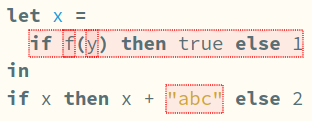
\includegraphics[scale=0.5]{images/hazel-intro-screenshot-v3.png}
\end{center}
\vspace{-3px}
A type checker with no support for error localization or recovery---%
as students in an undergraduate course might write---%
would simply report that this program is ill-typed. 
A more practical approach, and one common even in production type checkers, 
is to localize the first error that causes local type inference to fail and emit an explanatory error message before terminating.
In this example, the system might report that the variable \li{f} located on Line 2 is free, then terminate.

An implementation with support for type error recovery, like Elm's compiler or OCaml's \li{merlin} \cite{bour2018merlin}, would 
 be tasked with continuing past this first error.
 The general difficulty here is that there is now missing semantic information, namely the type of \li{f}, that 
 the bidirectional type system as specified 
 would appear to demand in order to proceed, here in order to determine which type the argument, \li{y}, is to be analyzed against. 
 Intuitively, however, it is clear that this knowledge is \emph{unnecessary} to make an error localization decision about \li{y}: 
it is free, so a second error can be simultaneously localized despite the missing information about \li{f}. 

To recover further, we might choose to also ignore the bidirectional type system's demand that the conditional guard be confirmed to be a boolean expression 
(because the type of \li{f(y)} is also not well-defined) 
and continue into its branches, observing that they have inconsistent types, \li{Bool} and \li{Int}. 
There are several ways to localize this error. 
One approach, taken e.g. by Elm and \li{merlin}, would be to assume, arbitrarily, that one branch is correct, localizing the error to the other branch. 
Heuristics have been developed to help make this choice less arbitrary, e.g. 
by observing recent editing history \cite{steady-typing}, 
or training a machine learning model \cite{SeidelBlame}. 
A less \emph{ad hoc} approach, which Hazel takes above, is to localize the inconsistency to the conditional as a whole, reporting that the problem is that the branch types differ. When the cursor is on this conditional expression, the Hazel type inspector---a status bar that reports typing information, including error messages, about the term at the cursor \cite{potter2020hazel}---displays:

\begin{center}
  
\includegraphics[width=0.9\textwidth]{images/haz3l-inconsistent-branches-cursor-inspector.png}
\end{center}

This localization decision affects how the system recovers as it proceeds into the let body. 
If localization had assumed that the \li{then} branch were correct, as for example in \li{merlin}, then 
\li{x : Bool} and an error should be reported on only the second use of \li{x}. 
If the \li{else} branch were chosen, then \li{x : Int} and an error would be reported on only the first use of \li{x}. 
 In either case, this error might mislead the programmer if the earlier localization guess was incorrect.
If the inconsistency were localized to the conditional expression as a whole, as in Hazel, then we again confront the problem of missing type information: 
\li{x} does not have a known type,
though it \emph{is} known to be bound. 
There is no definitive type or binding error at either use of \li{x}, 
so we do not report an error in Hazel. More specifically, we treat \li{x}'s type as the unknown a.k.a. dynamic type from gradual typing \cite{Siek06a}.
In any of these cases, we would like to be able to recover and 
localize the type inconsistency on the string addend because the \li{+} operator is integer addition in Hazel.
Recovering from this error, we can assume that both branch types in the second conditional will have \li{Int} type, so no 
error is marked on the conditional as a whole.

This informal exercise demonstrates that (1) localization choices can vary, particularly with regard to the extent to which they make \emph{ad hoc} guesses about intent;  
(2) when combined with error recovery, one localization decision can influence downstream localization decisions; and 
(3) error recovery necessitates reasoning without complete knowledge about types and binding. We argue that such semantic subtleties call for a rigorous theoretical treatment of these topics.

\Cref{sec:calculus} of this paper develops the first comprehensive {type-theoretic formulation} of type error localization and recovery, called the \emph{marked lambda calculus}.
We bring together three individually well-studied ideas: (1) bidirectional typing, which specifies how type and binding information flows from 
type annotations to expressions \cite{Localinf,BidirTyping}, (2) gradual typing, which offers a principled approach for recovering from missing type information \cite{Siek06a,siek2015refined}, and 
(3) non-empty holes, which function as syntactic membranes marking erroneous terms \cite{HazelnutPOPL}, operationalizing the ``red lines'' that an editor displays.
The marked lambda calculus achieves \emph{total error recovery}, meaning that \emph{every} syntactically well-formed program sketch (a program structure with, optionally, empty holes \cite{solar2013program}) can be marked, i.e. its errors can be simultaneously localized, such that the resulting program has a well-defined type and binding structure.
We establish this and other properties as metatheorems that we mechanize in the Agda proof assistant. 
As we define the calculus, we consider a number of situations where error localization decisions are subtle and conclude by defining some extensions of the intentionally minimal core calculus, e.g. with destructuring patterns and System F-style polymorphism, 
that serve as case studies of the general approach that we hope this paper will be adopted by language designers defining practical type systems.

\Cref{sec:calculus-hazel} describes our own effort in this direction, which is to scale up the marked lambda calculus as the new basis for Hazel, a typed functional programming environment that fully solves the semantic gap problem: Hazel's semantic services are available as long as the program sketch is syntactically well-formed. Prior work has separately considered mechanisms for maintaining syntactically well-formed program sketches during development: manual hole insertion (as in Agda \cite{norell:thesis}, GHC Haskell \cite{haskell-holes}, Idris \cite{DBLP:journals/jfp/Brady13}, and others), syntax error recovery \cite{medeiros20,sorkin11}, and structure editing \cite{HazelnutPOPL,teitelbaum_cornell_1981}. 
Hazel has both a textual syntax and a structure editor \cite{HazelnutPOPL,DBLP:conf/vl/Moon023}. 
%offering (1) a textual syntax, which allows the programmer to manually insert empty holes as necessary, (2) a text-like structure editor that offers partial syntax error recovery (inserting holes to maintain well-formedness as long as all matching delimiters have been placed) \cite{tylr}, and (3) a term-based structure editor with total syntax error recovery, i.e. a guarantee that every edit maintains syntactic well-formedness \cite{HazelnutPOPL}\todo{popl17}. 
As a secondary contribution, 
\cref{sec:calculus-hazelnut} describes how (1)  total marking can resolve the problem of undefined behavior in the Hazelnut structure editor calculus, 
and (2) integrating marking with typed structure editing allows us to incrementally re-mark only where necessary based on the edit location and the type and binding structure.

% which include type hints \cite{potter1}, semantic navigation, semantic code completion \cite{potter1,blinn}, contextualized documentation \cite{potter2}, and, because Hazel is able to evaluate programs with empty and non-empty holes due to prior work \cite{HazelnutLive}, even semantic services that require run-time information, like live testing, 
% 

The developments in Section~\ref{sec:calculus} support the intuition (remarked upon by \citet{Localinf} and \citet{BidirTyping}) that local type inference pairs well with type error localization and recovery because information flows systematically and locally through the tree. However, many functional languages including Elm, OCaml and Haskell feature constraint-based type inference, with constraints gathered globally. For type systems where inference is decidable, this is powerful, but it is also notorious for complicating error localization, because inconsistencies can arise through a confluence of constraints originating from any number of locations \cite{DBLP:conf/popl/Wand86}. 

For example, in the following Hazel expression (ignoring the error on the type hole for the moment), bidirectional error localization 
does not mark any uses of \li{x} as erroneous because a type for \li{x} cannot locally be inferred (the let-bound expression is an empty hole, which has unknown type). However, by gathering constraints from the three uses of \li{x} and attempting to unify, we see that the type hole is unfillable. Rather than arbitrarily privileging one of these uses, as is the case in languages like OCaml (and which has led to the development of complex heuristics, e.g. using machine learning \cite{SeidelBlame}, to avoid misleading programmers), this error is localized, with a \li{!}, to the type hole itself, with the error message providing partially consistent solutions as shown.
\begin{center}
\vspace{-3px}
    % 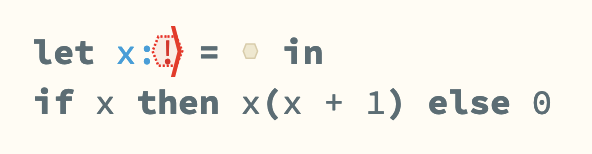
\includegraphics[scale=0.55]{images/intro-thi.png}
    % 
\includegraphics[scale=0.4]{images/example_CI.png}
    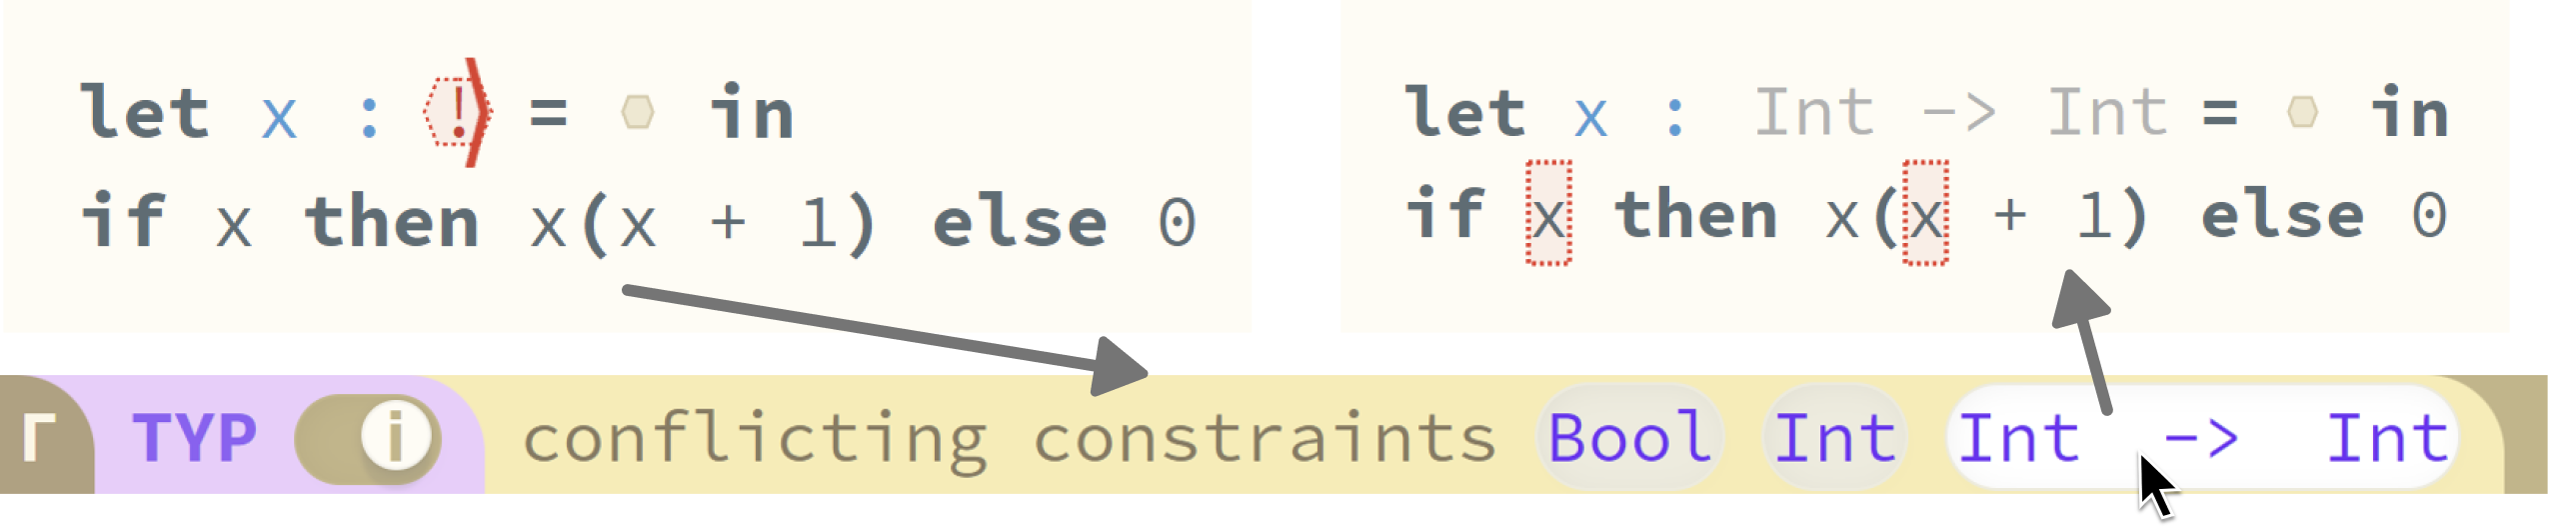
\includegraphics[scale=0.4]{images/figSugg.png}
\end{center}


The user can interactively explore possible error localizations by hovering over a partially consistent suggestion, which (temporarily) fills the type hole and thus returns the localization decision to the local inference system.
Here, each choice causes a different set of two uses of \li{x} to be marked, e.g. the first and third use for \li{Int -> Int} (shown above). Until the choice is finalized, the type hole continues to operate gradually.
\cref{sec:thi} describes this distinctively neutral approach to blending local and constraint-based type inference in Hazel, where local inference is used to systematically mark erroneous expressions in the program and constraint-based inference (using entirely standard algorithms, which we do not repeat in this paper) is used exclusively to locate unfillable holes.
